% !TeX spellcheck = sv_SE
\documentclass[a4paper]{IEEEtran}
\def\thepage{} %a4paper adds page numbers, this fix removes them

\usepackage[pdftex]{graphicx}
\usepackage[T1]{fontenc}
\usepackage[utf8]{inputenc} 

\usepackage[swedish]{babel}

\usepackage{url}
\makeatletter
\g@addto@macro{\UrlBreaks}{\UrlOrds}
\makeatother

\usepackage{scrextend}

\hyphenation{inne-bär}

\title{Autonomous Vehicles}
% http://www.software-center.se/digitalAssets/1521/1521374_kent-sw-center---software---need-for-speed.v001.pdf
% 1. Teknisk översikt
% 2. Nutida tillämplingar
% 3. Framtida och möjliga tillämpningar
% 4. Konkurrerande teknologier och standarder. Fördelar och nackdelar
% 5. Egna slutsatser

\author{\IEEEauthorblockN{Niklas Hedström, Emil Wihlander\\ }
\IEEEauthorblockA{Lunds Tekniska Högskola\\
Lund, Sverige\\
Email: \{dat15ewi, dat15nhe\}@student.lu.se}}

%----------------------------------------------------------------

\begin{document}
\maketitle

\begin{abstract}

\end{abstract}


\section{Introduktion}
\emph{Autonomous vehicles}, eller \emph{självkörande fordon}, är fordon som på ett eller annat sätt kan styra sig själv baserat på omgivningen. 
\emph{SAE International} har definierat klassificeringsnivåer som inom industrin har blivit allmänt accepterade där fordon klassas från SAE level 0 - Ingen automatisering, till SAE level 5 - Fullt automatiserad. \cite{SAE2014} 

Denna rapport kommer behandla den kommunikation som behöver ske för att självkörning ska kunna fungera, det innebär både intern och extern kommunikation. 
Det inkluderar teknologier som redan är standardiserade och välanvända samt potentiella teknologier som idag inte är färdigutvecklade men ger möjligheten att lösa problem som idag saknar en universellt använd lösning.

Huvudfokus kommer ligga på \emph{självkörande bilar} snarare fordon då det finns ett stort intresse både bland klassiska biltillverkare så som Volvo, Mercedes-Benz och Ford och nya företag inom bilbranschen så som Google, Tesla och Uber att vara först ut. 
Den konkurrenspräglade miljön innebär att företagen har varit öppna om sina framsteg inom området och har därmed publicerat mycket information. \cite{VolvoAD,MercedesAD,FordAD,GoogleAD,TeslaAD,UberAD}

\section{Klassificering}
\emph{SAE international standard J3016} definierar de olika nivåerna av självkörning enligt: \cite{SAE2014}

\vspace{10 pt}
\begin{labeling}{nivå 1}
	\item [\textbf{nivå 0}] \emph{No Automation}. Fordonet saknar helt självkörning. Kan skicka varningar till föraren, men är inget krav.
	\item [\textbf{nivå 1}] \emph{Driver Assistance}. Fordonet har vissa funktioner som påverkar det baserat på omgivningen. T.ex. ACC (Adaptive Cruise Control)\footnote{När fordonet kan ändra farthållaren baserat på hastigheten av framförvarande fordon\cite{ACC}}, LKA (Lane Keeping Assistance)\footnote{När fordonet kan hjälpa till att styra så att den håller sig inom nuvarande fil\cite{LKA}} och Parkeringshjälp\footnote{När fordonet hjälper till att parkera genom att ta över styrningen\cite{AP}}. Föraren måste dock alltid vara redo att ta över.
	\item [\textbf{nivå 2}] \emph{Partial Automation}. Fordonet kan själv manövrera sig i kända förutsättningar, men när förutsättningar inte längre uppfylls måste föraren ta över genast.
	\item [\textbf{nivå 3}] \emph{Conditional Automation}. Fordonet ska utöver nivå 2 kunna hantera dynamiska situationer i specifika miljöer, så som huvudleder där gångtrafikanter saknas. Detta innebär att fordonet kör sig själv men kan fortfarande kräva att föraren tar när som helst.
	\item [\textbf{nivå 4}] \emph{High Automation}. Fordonet ska utöver nivå 3 kunna hantera situationer som inte förväntas uppstå och kunna agera därefter.
	\item [\textbf{nivå 5}] \emph{Full Automation}. Fordonet ska utöver nivå 4 kunna hantera alla miljöer och därmed aldrig kräva input från en potentiell förare.
\end{labeling}

\section{Nuvarande Implementation}
Begreppet självkörande bil brukar bland vanliga konsumenter syfta på att bilen har en nivå på 4 och uppåt och det finns inget ute på marknaden som uppfyller det nu.
Teslas Autopilot, som funnits ute på marknaden i några år, brukar klassas som någonstans mellan nivå 2 och 3 då den bland annat har en kombination av ACC och LKA. 
Googles självkörande bilar är nivå 4 då de saknar både ratt och gas- och bromspedal men klarar av få miljöer.
Dessa finns dock inte ute på marknaden.
Uber lanserade under hösten 2016 modifierade bilar från Ford och Volvo med nivå 4 som används som taxibilar i Pittsburg, CA, USA. Då dessa är mod konsumenter sitter det dock alltid en observatör som övervakar att systemet fungerar rätt.
Volvo har som mål att lansera självkörande bilar med nivå 4 under 2017. Dessa ska ut till vanliga konsumenter utan att något för Volvo övervakar användandet. Det är dock på endast på några få huvudleder runt omkring Göteborg som självkörning kommer vara tillgänglig, på resterande vägar används bilen utan självkörning.
\cite{UberAD,VergeAD,CWGoogleAD}
\section{Teknisk bakgrund}
En elektrisk styrenhet, ECU (\emph{eng. electronic control unit}), är en microdator som används i bilar för att styra tidigare mekaniska delar för att förbättra bland annat precision och komfort. 
I samband med att ECU:er började bli en vital del för att förbättra bilupplevelsen krävdes ett system för att kommunicera mellan dem och det som blev de facto var CAN (Controller Area Network). (se sektion \ref{sec:CAN})

CAN är en buss som består av två protokoll som täcker lager 1 och 2 av OSI-modellen och utvecklades till att börja med av Bosch under 80-talet innan det 1992 fick en internationell standard och fördes över till den nystartade associationen \emph{CAN in Automation} för vidare utveckling. \cite{CANhist}

På senare år, i och med att antalet unika ECU:er i bilar har ökat markant och därmed mängden information som skickas, har konkurrenter till CAN uppkommit som klarar högre bandbredd och som är mer pålitliga. Den främsta är FlexRay och används av flera europeiska tillverkare och används tillsammans med CAN. \cite{FlexRayWiki} (se sektion \ref{sec:FlexRay})

När det kommer till kommunikation mellan bilar saknas fortfarande en gemensam, välanvänd standard. Ett konsortium mellan, bland andra, flera stora biltillverkare är ``CAR 2 CAR Communication Consortium''. De jobbar för att en gemensam standard i Europa och använder \emph{IEEE 802.11p} som är en vidareutveckling av \emph{IEEE 802.11} som är marknadsförs som Wi-Fi. En av styrkorna med teknologin är att noder (läs bilar, trafikljus, etc.) kan kommunicera direkt med varandra utan att kräva infrastruktur, så kallad D2D (\emph{Device To Device}) kommunikation. En stor nackdel med teknologin är dock räckvidden är kort och att fördröjningen kan bli lång i samband med trafikstockning. \cite{C2COrg,C2CDepl,ericsson5G,5GPPP}

Alternativ är att låta all information passera genom en central server över dagens mobilnät\footnote{Syftar på de nät som kan skicka data, det vill säga 3G och 4G}, D2I (\emph{Device To Infrastructure}) som tar hand om hur, och till vilka noder, datan ska skickas. Fördelar här är att data kan bearbetas och sammanställas av molnet men detta kräver att bilen alltid är uppkopplad mot internet vilket i sin tur kräver infrastruktur vilket kan vara problematiskt. \cite{VolvoSRA}

Ett sista alternativ är en hybrid mellan D2D och D2I. Det finns en vidareutveckling av LTE som kallas LTE ProSe (\emph{Long Term Evolution Proximity Services}) som ger möjligheten till D2D-kommunikation. Nästa generations mobilnätsstandard, 5G, förväntas också inkludera D2D från början samt höga överföringshastigheter, låg latens och bra pålitlighet. \cite{5GPPP,LTED2D}

Så för att sammanfatta skulle en självkörande bil inom de kommande åren kunna ha ett nät av ECU:er enligt figur \ref{Img:CarScheme}.
Bussen mellan alla stora delsystem är en FlexRay och bussen inom delsystem är CAN. Det finns ett delsystem som tar hand om att manövrera bilen, VCU, ett delsystem som tar hand om analysen av data (sensorer, kartor, information från andra noder) och bestämmer vad som ska hända, ADU, och ett delsystem som tar hand om den externa kommunikationen med andra noder och databaser, ECU. 
\begin{figure}
	\begin{center}
		\resizebox{!}{60mm}{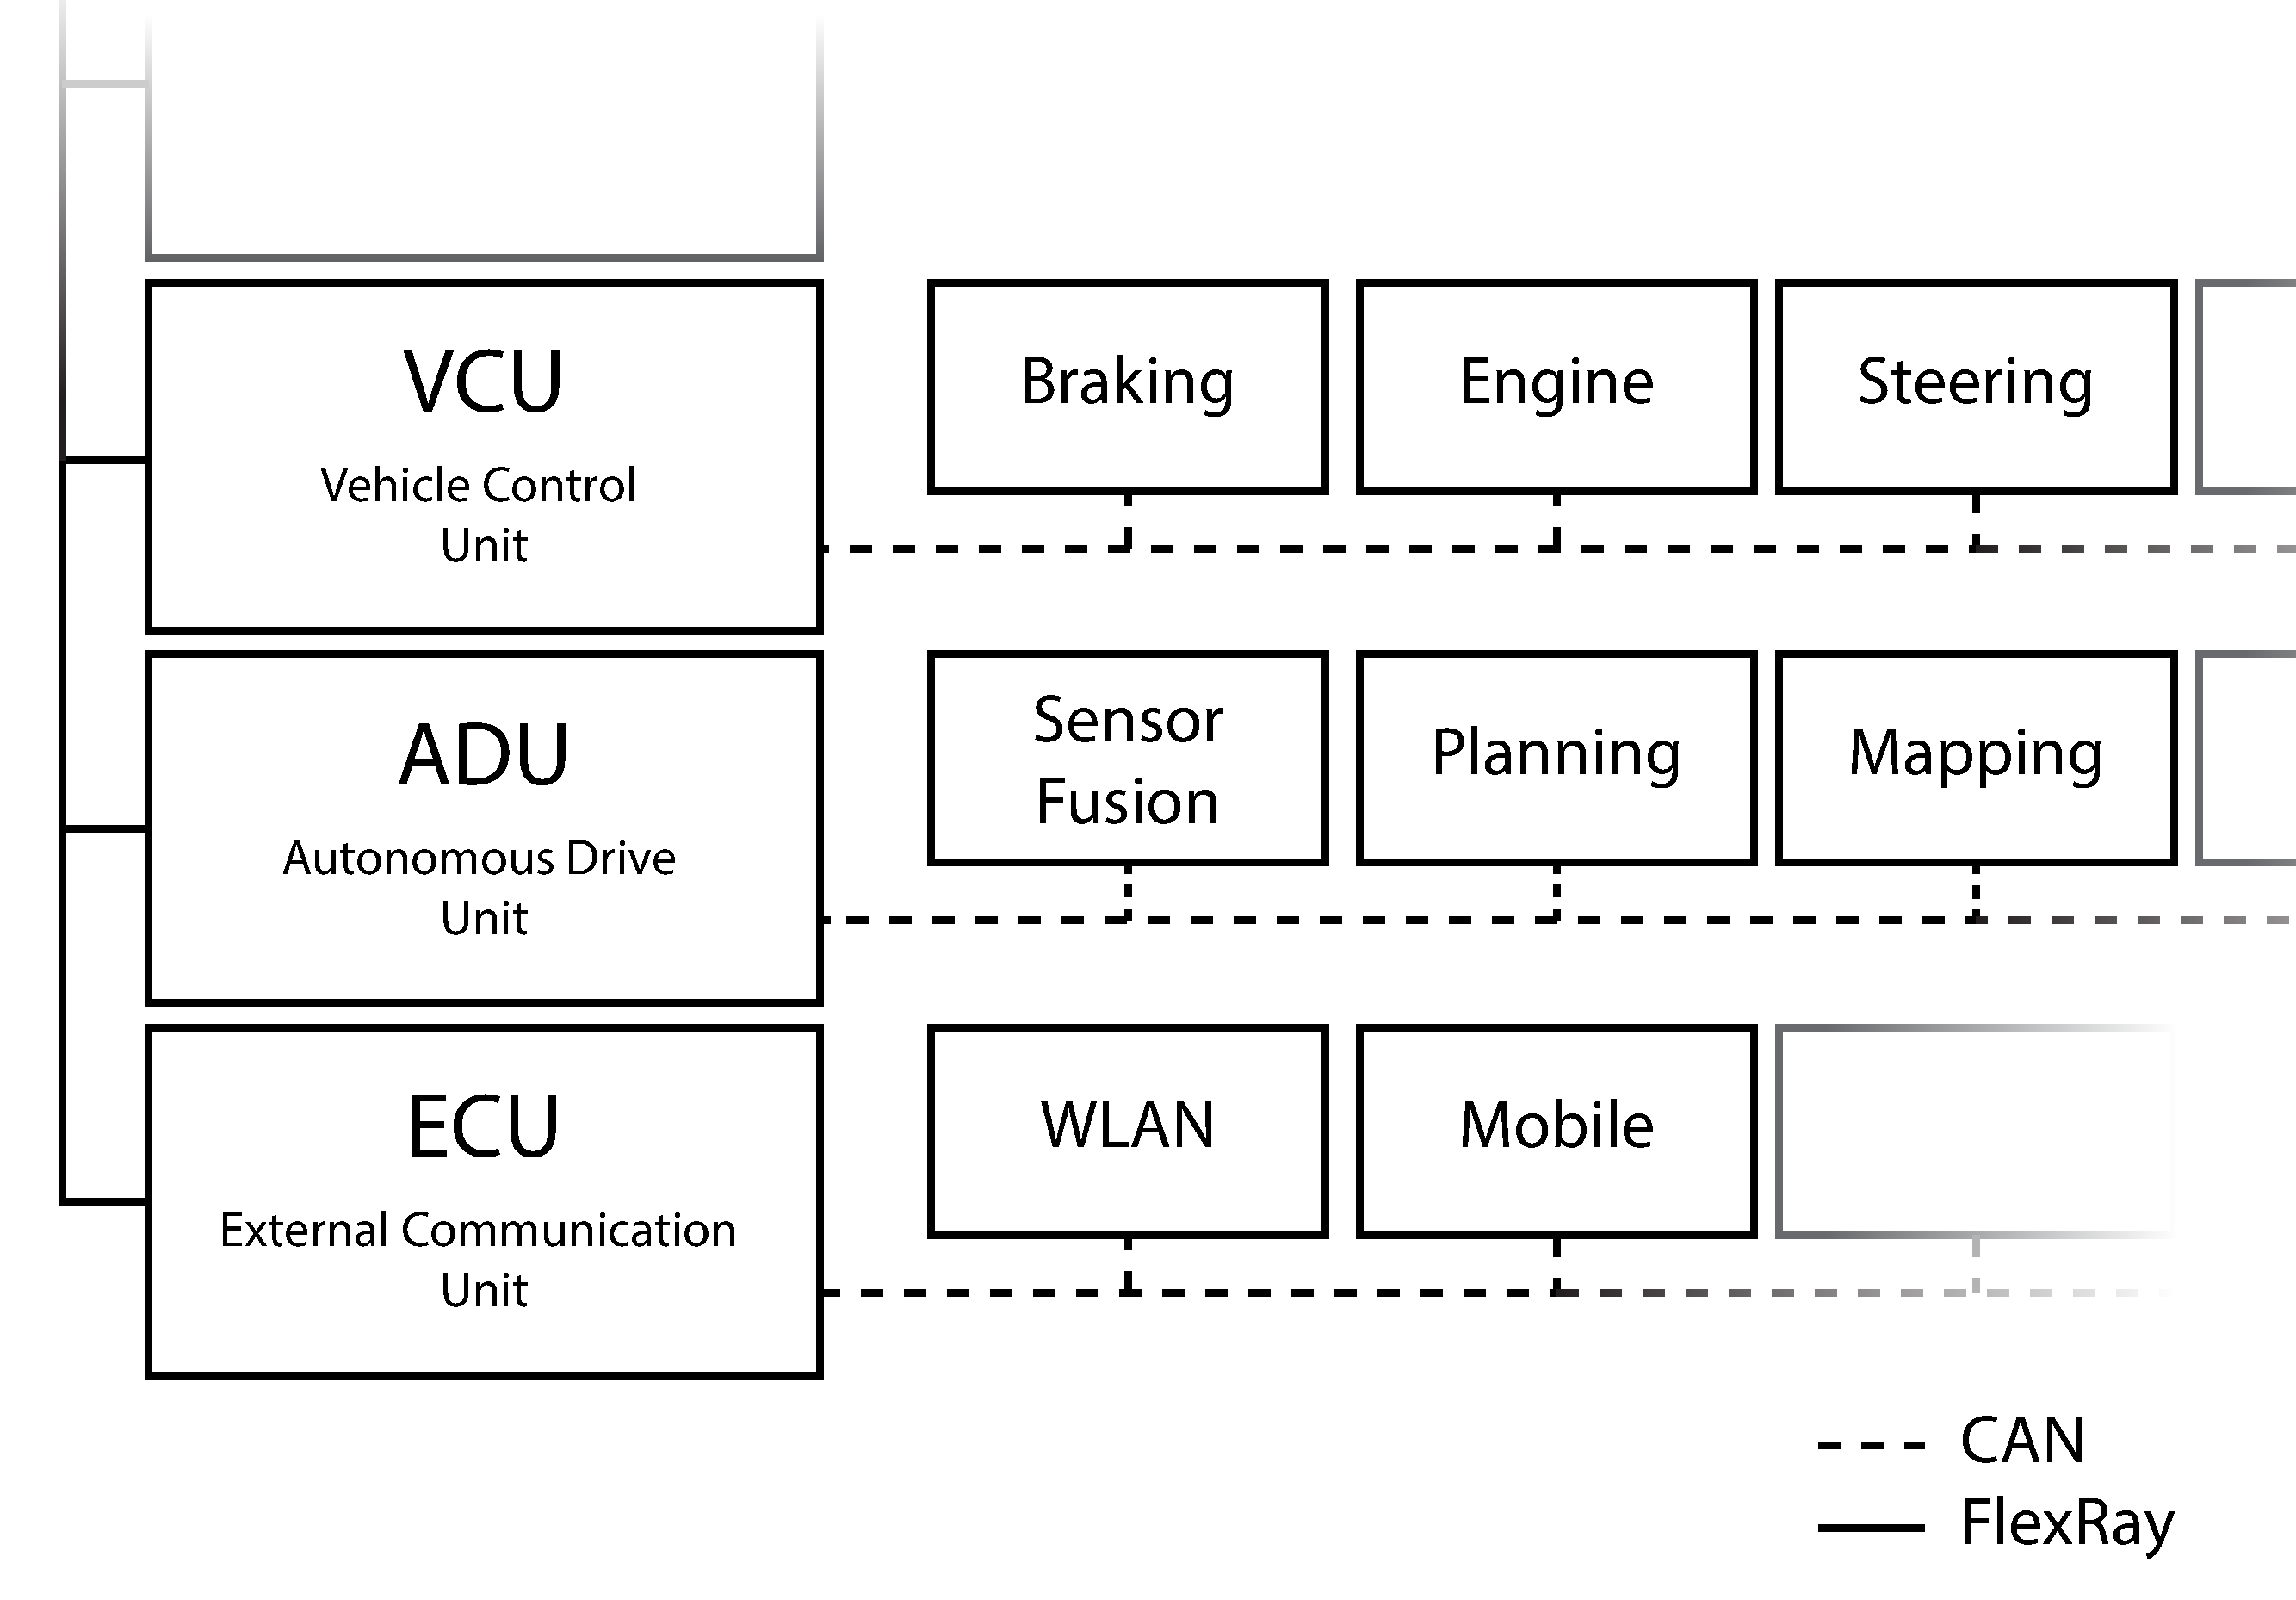
\includegraphics{CarCommunicationScheme.pdf}}
	\end{center}
	\caption{En förenklad modell över hur ett nät inuti en självkörande bil skulle kunna se ut. Delvis baserad på nätet över Volvo XC90 2015 \cite{xc90Scheme}}
	\label{Img:CarScheme}
\end{figure}

\section{Internal Vehicle Communication}

\subsection{Controller Area Network} \label{sec:CAN}
CAN (Controller area network) är en kommunikationsbuss utvecklad av företaget BOSCH som en multi-master, message broadcast system. Tillskillnad från USB och Ethernet sänder inte CAN-bussen stora datapaket från nod A till nod B (Point-to-Point) under uppsyn av en central buss ledare. I ett CAN-bus nätverk skickas information i en broadcast till hela nätverket, i till exempel en självkörande bil skickas många små meddelanden mellan olika ECU:er i en broadcast så att de olika meddelanden når alla nödvändiga ECU:er de vill säga datakonsekvens i varje nod i hela nätverkets. CAN-bussen är en ISO definierad seriell kommunikationsbuss. CAN-bussen har en hög immunitet mot elektrisk interfens och har en förmåga att göra självdiagnostik och reparera datafel. \cite{CANintr}

\subsubsection{Physical Layer}
Det fysiska lagret i CAN-Bussen består av tre sublager the physical coding (PCS) som är implementerat i CAN-bussens kontroll chip, the physical media attachment (PMA) som specificerar transceiverns egenskaper och the physical media-dependent sub-layers (PMS) som är programspecifik och är inte generellt standardiserad.

The physical coding sublagret i CAN-bussen använder sig av NRZ kodning, jämför med manchester kodning så behöver man inte med NRZ i varje bit ha en fallande eller stigande flank utan signalen kan hållas konstant över en längre period om de överförda bitarna har samma logiska värde. Således måste åtgärder vidtas för att försäkra sig om att det maximala tillåtna intervallet mellan två signalflanker inte överskrids. Detta är viktigt för synkroniseringen. Åtgärdens som gör är att CAN-bussen använder ett protokoll som gör att när det kommer fem bitar av samma värde lägger CAN-buss kontrollen in en bit av motsattvärde, även kallat ”bit stuffing”. Sedan gör den mottagande CAN-buss noden det motsatta och tar bort de instoppade bitarna.
Om bussen är inaktiv så används den första fallande flanken till att globalt synkronisera alla CAN-buss kontroller. 

The physical media attachment sublagret är normalt implementerat i transceiver chipet. Inputen är TxD och RxD signalerna från CAN-buss kontrollen och outputen driver busslinjerna. \cite{CANphys}

\subsubsection{Data Link Layer}
Datalänks lagret är uppgjord av två protokoll Classical CAN som introducerades 1986 och implementerades 1988 och CAN FD som lanserades 2012 och som blev internationellt standardiserad 2015 i ISO 11898-1. Strukturen av CAN-buss dataramar är samma för både Classical CAN och CAN FD bara fält detaljer är olika. Dataramen består av Start-of-frame (SOF), Arbitration field, Control field, Data field, cyclic redundancy check field (CRC), Acknowledegement field (ACK), End-of-frame (EOF) och Intermission field (IMF). 

Båda CAN protokollen har gemensamma funktioner. Varje nod har rätten att be om att överföra data när som helst (multi-master capability). Metoden för att undvika överförings kollisioner är samma för båda protokollen. De använder sig av prioriteringslista och det meddelandet med högst prioritet får skicka först. CAN-buss identifierare som är en del av meddelandet och indicerar prioriteten. Desto lägre nummer värde på identifieraren desto högre prioritet. Alla typer av ramar skickas vi en broadcast i CAN-bussen. 

The Classical CAN protokollet använder sig av en bithastighet i skilje och data fasen. Överföringshastigheten är begränsad till 1 MegaBit per sekund för korta nätverk. The payload för Classical CAN är begränsad till 8 bytes.

The CAN FD protokollet har en payload 64 bytes. Hastigheten för skilje fasen för CAN FD är den samma som för Classical CAN medans hastigheten för data fasen är begränsad av transcieverns egenskaper och oscillatorns tolerans. \cite{CANdata}

\subsection{FlexRay} \label{sec:FlexRay}
kommunikationsbussen är en feltolerant och höghastighets bussystem som är utvecklad i konsensus av biltillverkare och ledande leverantörer. 
FlexRay:en är jämfört med CAN-bussen mycket snabbare men mycket dyrare. 
FlexRay:en kan ha en payload som är mer än 30 gånger större än vad CAN kan hantera.

FlexRay protokollet är ett unikt tidsbestämt protokoll som ger möjligheter för deterministisk data som kommer in vid en förutsägbar tid nere på mikrosekund nivå, samt en CAN-buss liknande händelsedriven dynamisk data som hanterar mängd olika ramar. 
FlexRay:en lyckas med denna hybrid av både statiska och dynamiska ramar med en förutbestäm kommunikationskretslopp som ger en förutbestämt rum för statisk och dynamisk data. 

FlexRay:ens dataram består av ett huvud, själva datan och en svans. Huvudet är uppgjord av 40 bitar och har följande fält, status bitar (5 bitar), ram id (11 bitar), payload längd (7 bitar), huvud CRC (11 bitar) och cycle count (6 bitar). 
Själva datan kan vara upp till 256 bytes. Svansen är uppgjord av 24 bitar och det är tre stycken 8 bitars CRC fält som ska upptäck fel. \cite{FlexRayOverview}

\section{External Vehicle Communication}
\subsection{Cloud to Car Communication}
Eftersom access till internet är ett krav om en biltillverkares bilar ska kunna komma åt dess molntjänst är dagens mobilnät väl anpassade för detta syftet då länder med välutvecklad infrastruktur har täckning över näst intill hela landet. 
Eftersom det skickas över internet används IP (\emph{Internet Protocol}) som nätverksprotokoll och IP-paket kommer då skickas mellan bilar och molnet. 
Informationen som skickas kan innehålla konfidentiell data så som position, detta innebär att applikations protokollet som används antagligen använder någon typ av kryptering.

Eftersom fördröjningen redan är relativt hög om data ska gå mellan två bilar används denna lösningen inte till tidskritiska applikationer så som att undvika kollision. 
Det innebär att transportprotokollet som används antagligen värderar att data kommer fram högre än låg fördröjning. 
Detta skulle exempelvis kunna vara TCP (\emph{Transmission Control Protocol}) som kommer skicka om alla paket som inte konfirmerats att det kommit fram. \cite{TCP}

I Europa finns det en standard för att koda bilrelaterad data kallad DATEX \textrm{II}. 
Denna använder XML (\emph{Extensible Markup Language}) för att koda data och HTTP (\emph{HyperText Transfer Protocol}) är ett vanligt applikationsprotokoll för att skicka XML över  internet.
Eftersom kryptering dock är en vital del för typen av data som skickas används troligtvis HTTPS istället. 
HTTPS bygger på HTTP men med tillägget att det använder TLS (\emph{Transport Layer Security}) för att bland annat kryptera data och försäkra integritet mellan bil och server. \cite{DATEXII,HTTPS,TLS}

\subsection{Car to Car Communication}
\subsubsection{IEEE 802.11p}
IEEE 802.11p eller WAVE (\emph{Wireless Access in Vehicular Environments}) är en underkategori till IEEE 802.11 som vanligtvis brukar kallas för Wi-Fi. 
WAVE utnyttjar på det fysiska lagret OFDM (\emph{Orthogonal Frequency Division Multiplexing}) och är uppdelat på flera band på 10~MHz var vid 5.9~GHz. 
Ett av banden är en så kallad \emph{Control Channel} och all D2D kommunikation förväntas gå över detta bandet. 
WAVE använder CSMA/CA (\emph{Carrier Sense Multiple Access with Collision Avoidance}) som accessmetod, detta tillsammans med den ensamma kanalen innebär att i samband med att trafiken ökar så ökar fördröjningen eftersom CSMA/CA ökar väntetiden på att skicka meddelanden logaritmiskt om kanalen är upptagen.
Ett annat problem med CSMA/CA är om noder inte syns, se figur \ref{Img:HiddenNode}. %bild på det
Det innebär att en nod kan tro att meddelandet kom fram ostört men egentligen fungerade det inte.

\begin{figure}
	\begin{center}
		\resizebox{!}{60mm}{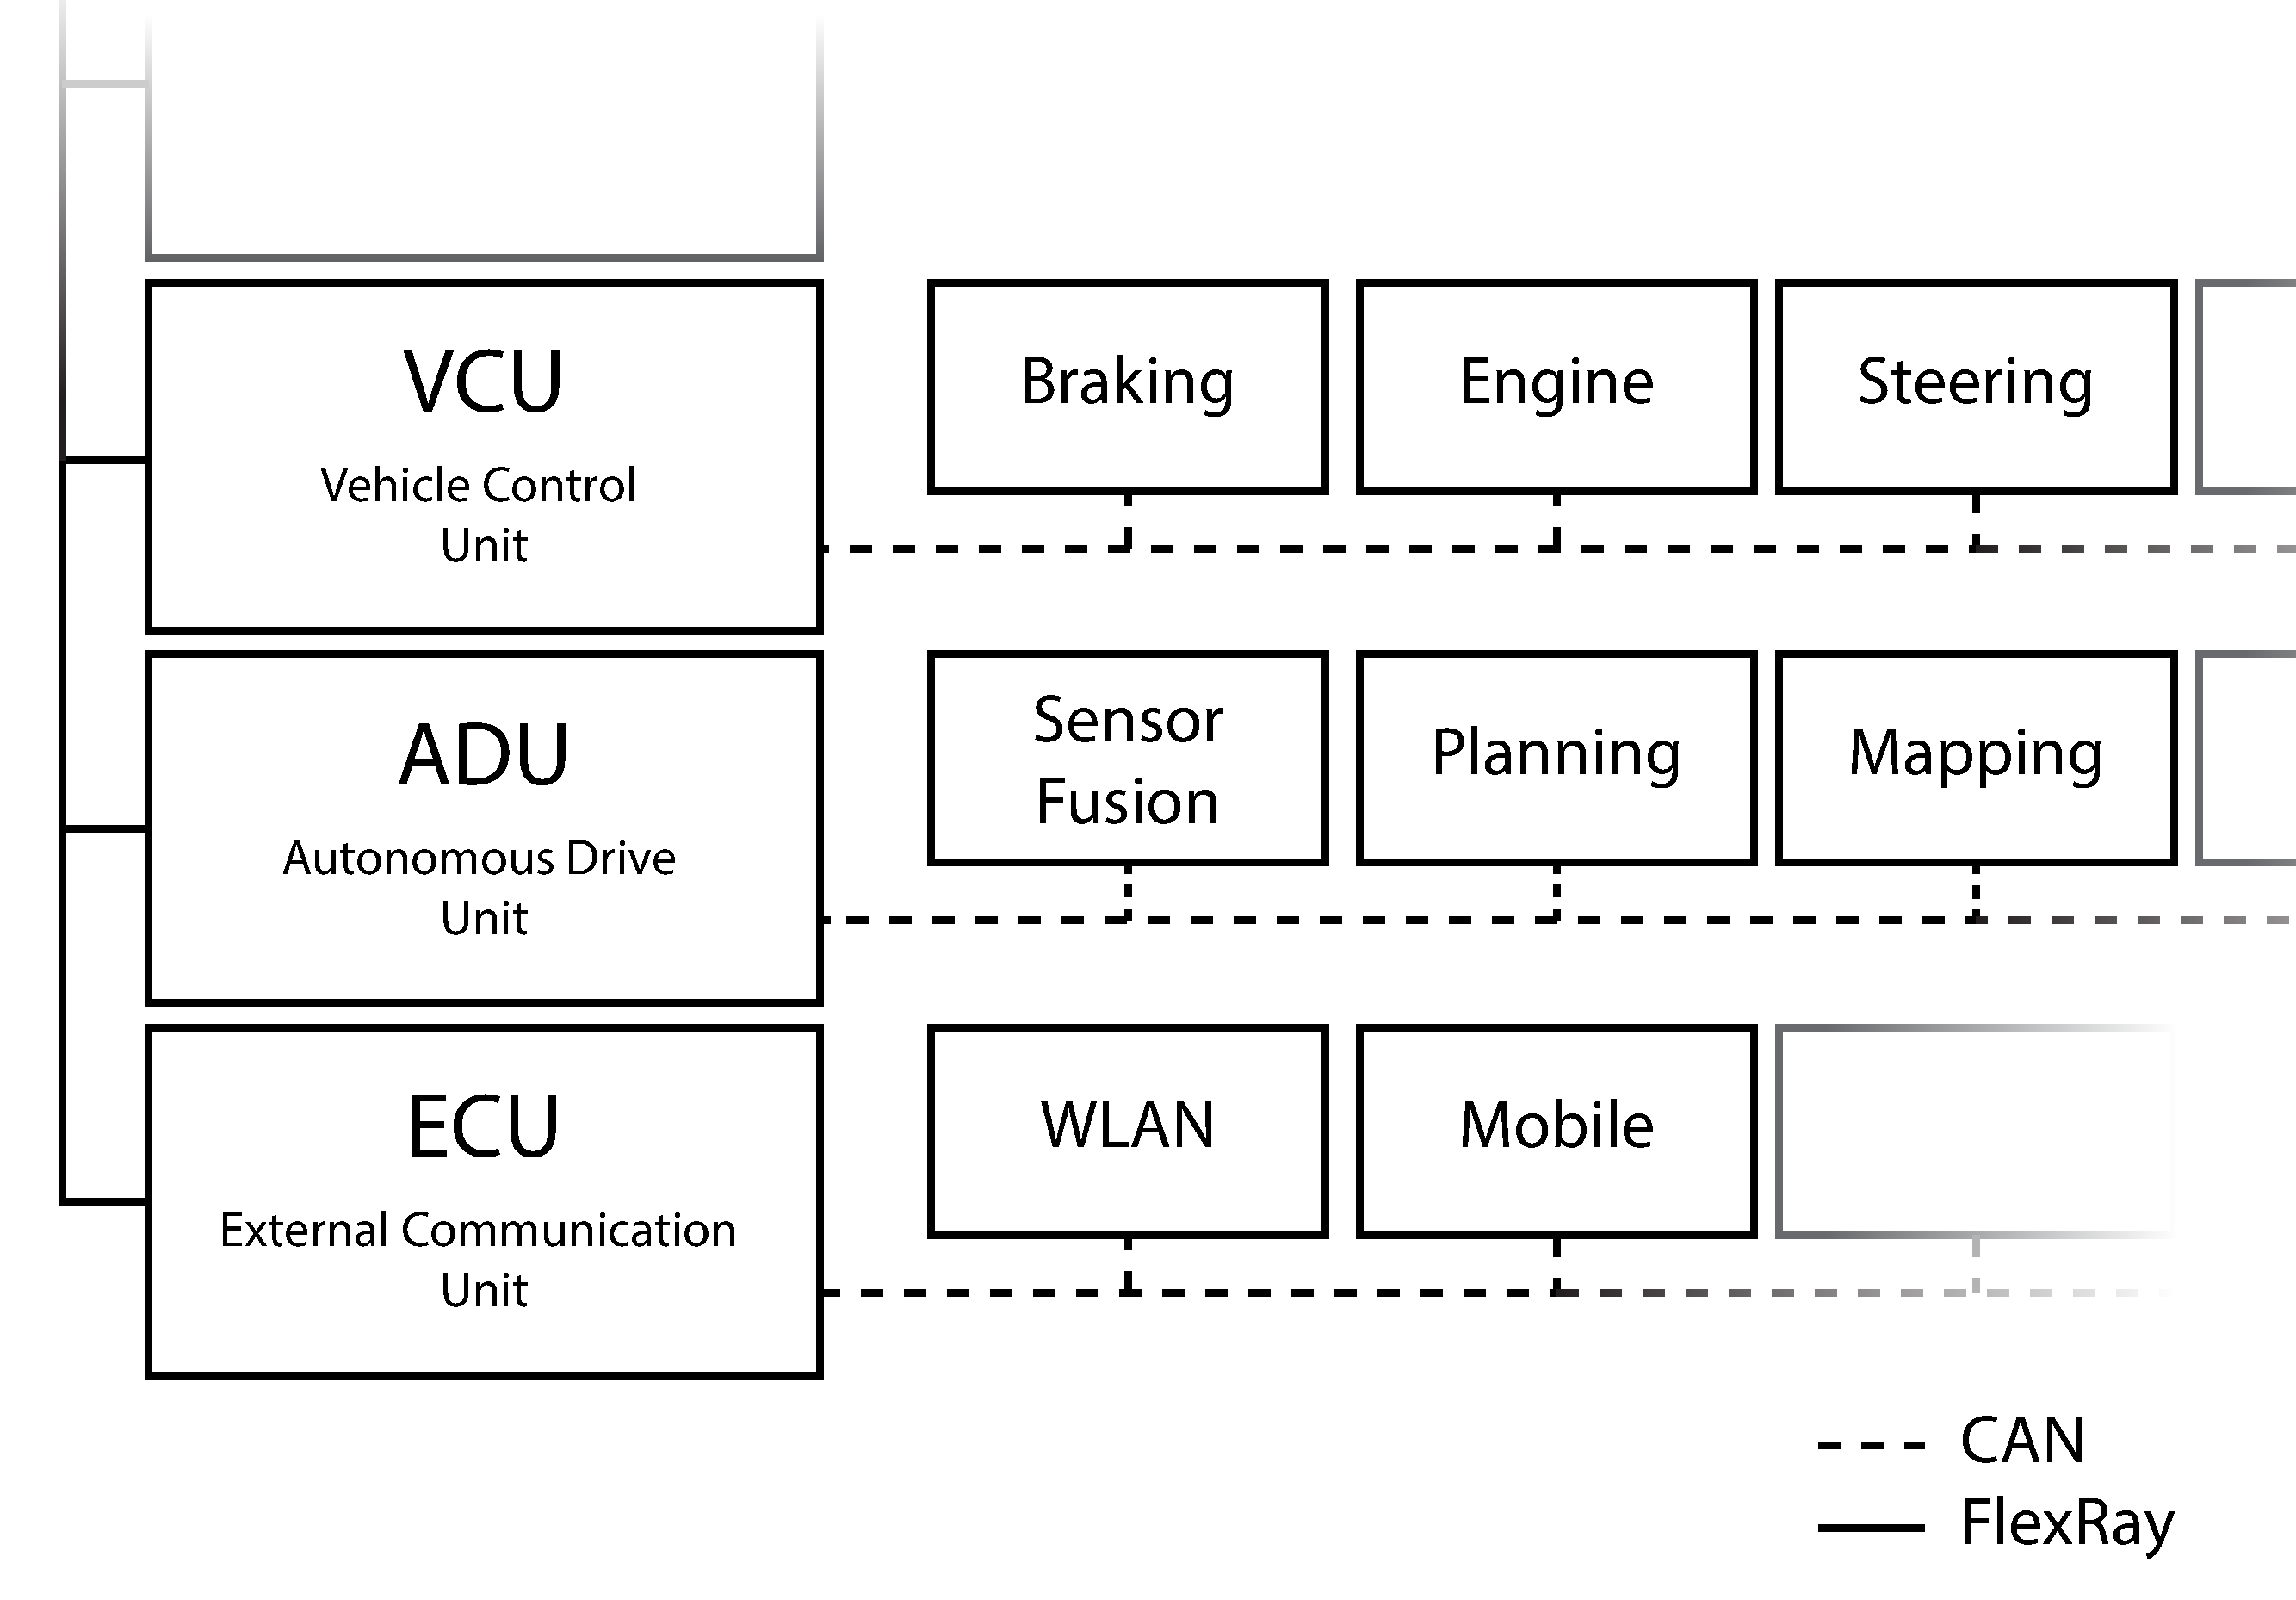
\includegraphics{CarCommunicationScheme.pdf}}
	\end{center}
	\caption{Visualisering av problemet när noder inte syns för sändare av meddelanden.}
	\label{Img:HiddenNode}
\end{figure}

På grund av de fysiska egenskaperna av 5.9~GHz-bandet så är räckvidden som mest en halv kilometer och det är därför inte en rimlig lösning för applikationer där ett krav på längre avstånd är ett måste. 
En typisk miljö som är problematisk är motorvägar då de höga hastigheterna gör att tidsskillnaden mellan bilar på 500 meters avstånd inte är speciellt stor. \cite{5GPPP}
\subsubsection{LTE ProSe}
LTE ProSe (\emph{Long Term Evolution Proximity Services}) är en vidareutveckling av LTE som utöver när noden har E-UTRAN-täckning\footnote{Evolved Universal Terrestrial Radio Access Network är interfacet som används i LTE för att kommunicera mellan radiostationer och noder} även kan kommunicera direkt mellan noder.
Metoden som används i kommunikation mellan noder är SC-FDMA (\emph{Single-Carrier Frequency-Division Multiple Access}), vilket är samma som används i uplink till radiostationer. Det finns två lägen:
\begin{enumerate}
	\item Noderna är uppkopplade mot en radiostation och radiostationen modererar när noderna får skicka meddelanden till varandra så meddelanden aldrig krockar.
	\item Noderna saknar uppkoppling och väljer själva på vilket band och när de skickar meddelandena.
\end{enumerate}
Läge 2 ger liknande problem som CSMA/CA då trafik kan krocka och meddelanden kan inte försäkras att de skickas inom ett visst tidsspann.
Men eftersom E-UTRAN-täckning i trafiktunga områden ofta finns löser läge 1 problemen som uppstår i IEEE 802.11p.
Eftersom samma modul används för både LTE och LTE ProSe kan teknikerna varieras med varandra så den bästa lösningen för olika problem kan användas.
LTE ProSe är dock inte designat för V2X-kommunikation (Vehicle To Everything) så det saknar stöd för protokoll och säkerhetslager som denna typen av kommunikation kräver.
\subsubsection{5G}
5G är nästa generations mobila kommunikationsstandard och är inte färdigställd än. Många lovande funktioner för V2X-kommunikation väntas dock så som låg fördröjning, hög pålitlighet och support för högre anslutningstäthet.
Det kommer inkludera D2D-kommunikation från början och täcka ett stort spektrum av nätverksband så både kommunikation mellan bilar nära varandra och långt ifrån varandra är stabil.
5G är alltså en god kandidat till att bli standarden för denna typen av kommunikation, men eftersom varken standarden eller faktisk hårdvara som utnyttjar den är färdig utvecklad finns en viss osäkerhet.

\section{Slutsats}
Utvecklingen av självkörande bilar är fortfarande i ett tidigt stadium. Internt i bilen kan dock gamla standarder användas då elektrifiering av bilar pågått under en längre tid och självkörning bara är en vidareutveckling av det. När det kommer till extern kommunikation är det dock fortfarande mycket som är oklart. Biltillverkarna är fortfarande inte överens när det kommer till en gemensam standard men för hoppningen är att 5G ska kunna förena biltillverkarna.






\begin{thebibliography}{77}
	\bibitem{SAE2014}SAE International: \emph{Automated Driving}, 
	\url{http://www.sae.org/misc/pdfs/automated_driving.pdf}, 
	2014 (hämtad 2016-12-02)
	
	\bibitem{VolvoAD}Volvo: \emph{Volvo Cars presents a unique solution for integrating self-driving cars into real traffic}, 
	\url{https://www.media.volvocars.com/global/en-gb/media/pressreleases/158276/volvo-cars-presents-a-unique-system-solution-for-integrating-self-driving-cars-into-real-traffic}, 
	2015-02-19 (hämtad 2016-12-02)
	
	\bibitem{MercedesAD}Mercedes: \emph{The Mercedes-Benz F 015 Luxury in Motion.}, 
	\url{https://www.mercedes-benz.com/en/mercedes-benz/innovation/research-vehicle-f-015-luxury-in-motion/}
	(hämtad 2016-12-02)
	
	\bibitem{FordAD}Ford: \emph{Ford börjar testa självkörande bilar i Europa under 2017}, 
	\url{http://www.mynewsdesk.com/se/ford/pressreleases/ford-boerjar-testa-sjaelvkoerande-bilar-i-europa-under-2017-1670717}, 
	2016-11-29 (Hämtad 2016-12-02)
	
	\bibitem{GoogleAD}Google: \emph{Google Self-Driving Car Project}, 
	\url{https://www.google.com/selfdrivingcar/} 
	(hämtad 2016-12-02)
	
	\bibitem{TeslaAD}Tesla: \emph{All Tesla Cars Being Produced Now Have Full Self-Driving Hardware}, 
	\url{https://www.tesla.com/blog/all-tesla-cars-being-produced-now-have-full-self-driving-hardware}, 
	2016-10-19 (hämtad 2016-12-02)
	
	\bibitem{UberAD}Uber: \emph{Pittsburgh, your Self-Driving Uber is arriving now}, 
	\url{https://newsroom.uber.com/pittsburgh-self-driving-uber/}, 
	2016-09-14 (hämtad 2016-12-02)
	
	\bibitem{ACC}Wikipedia: \emph{Autonomous cruise control}, 
	\url{https://en.wikipedia.org/wiki/Autonomous_cruise_control_system}, 
	2016-12-01 (Hämtad 2016-12-01)
	
	\bibitem{LKA}Toyota: \emph{Lane Keeping Assist}, 
	\url{http://www.toyota-global.com/innovation/safety_technology/safety_technology/technology_file/active/lka.html}
	(Hämtad 2016-12-01)
	
	\bibitem{AP}Wikipedia: \emph{Automatic parking}, 
	\url{https://en.wikipedia.org/wiki/Automatic_parking}, 
	2016-11-24 (Hämtad 2016-12-01)
	
	\bibitem{VergeAD}J. Golson: \emph{Volvo autonomous car engineer calls Tesla’s Autopilot a ‘wannabe'},
	\url{http://www.theverge.com/2016/4/27/11518826/volvo-tesla-autopilot-autonomous-self-driving-car},
	2016-04-27 (hämtad 2016-12-06)
	
	\bibitem{CWGoogleAD}D. Storm: \emph{Did you know Google's self-driving cars can't handle 99\% of roads in the US?},
	\url{http://www.computerworld.com/article/2599426/emerging-technology/did-you-know-googles-self-driving-cars-cant-handle-99-of-roads-in-the-us.html},
	2014-08-28 (hämtad 2016-12-06)
	
	\bibitem{CANhist}CAN in Automation (CiA): \emph{History of CAN technology},
	\url{https://www.can-cia.org/can-knowledge/can/can-history/}
	
	\bibitem{FlexRayWiki}Wikipedia: \emph{FlexRay},
	\url{https://en.wikipedia.org/wiki/FlexRay},
	2016-10-04 (hämtad 2016-12-04)
	
	\bibitem{C2COrg}CAR 2 CAR: \emph{Organisation},
	\url{https://www.car-2-car.org/index.php?id=22}
	(hämtad 2016-12-05)
	
	\bibitem{C2CDepl}CAR 2 CAR: \emph{Deployment of V2X services based on ITS-G5},
	\url{https://www.car-2-car.org/index.php?eID=tx_nawsecuredl&u=0&g=0&t=1480979291&hash=668c1e8c7a38f3d6229fb9d9e196f14fcbd1152e&file=fileadmin/downloads/PDFs/CAR_2_CAR_Communication_Consortium_Statement_ITSG5.pdf},
	2016-07-20 (hämtad 2016-12-05)
	
	\bibitem{ericsson5G}G. Fodor: \emph{D2D Communications – What Part Will It Play in 5G?},
	\url{https://www.ericsson.com/research-blog/5g/device-device-communications/},
	2014-07-10 (hämtad 2016-12-05)
	
	\bibitem{5GPPP}The 5G Infrastructure Public Private Partnership: \emph{5G Automotive Vision},
	\url{https://5g-ppp.eu/wp-content/uploads/2014/02/5G-PPP-White-Paper-on-Automotive-Vertical-Sectors.pdf},
	2015-10-20 (hämtad 2016-12-04)
	
	\bibitem{VolvoSRA}Volvo: \emph{Live smarter by sharing},
	\url{http://www.volvocars.com/intl/about/our-innovation-brands/sensus/live-smarter-by-sharing}
	(hämtad 2016-12-05)
	
	\bibitem{LTED2D}J. Schlienz, A. Roessler: \emph{Device to Device Communication in LTE},
	\url{https://cdn.rohde-schwarz.com/pws/dl_downloads/dl_application/application_notes/1ma264/1MA264_0e_D2DComm.pdf}
	(hämtad 2016-12-05)
	
	\bibitem{xc90Scheme}K. Niesel: \emph{Volvo Car Software Center Day}, 
	\url{http://www.software-center.se/digitalAssets/1521/1521374_kent-sw-center---software---need-for-speed.v001.pdf},
	s. 2 (hämtad 2016-12-04)
	
	\bibitem{CANintr}S. Corrigan: \emph{Introduction to the Controller Area Network (CAN)},
	\url{http://www.ti.com/lit/an/sloa101a/sloa101a.pdf},
	2008-07 (hämtad 2016-12-05)
	
	\bibitem{CANphys}CAN in Automation (CiA): \emph{CAN physical layer},
	\url{https://www.can-cia.org/can-knowledge/can/systemdesign-can-physicallayer/}
	(hämtad 2016-12-04)
	
	\bibitem{CANdata}CAN in Automation (CiA): \emph{CAN data link layers in some detail},
	\url{https://www.can-cia.org/can-knowledge/can/can-data-link-layers/}
	(hämtad 2016-12-04)
	
	\bibitem{FlexRayOverview}National Instruments: \emph{FlexRay Automotive Communication Bus Overview},
	\url{http://www.ni.com/white-paper/3352/en/},
	2016-08-24 (hämtad 2016-12-04)
	
	\bibitem{TCP}Information Sciences Institute	University of Southern California: \emph{Transmission Control Protocol},
	\url{https://tools.ietf.org/html/rfc793},
	1981-09 (hämtad 2016-12-08)
	
	\bibitem{DATEXII}DATEX: \emph{DATEX II XML Schema 2.2},
	\url{http://www.datex2.eu/content/datex-ii-xml-schema-22},
	2013-05-22 (hämtad 2016-12-08)
	
	\bibitem{HTTPS}The Internet Society: \emph{HTTP Over TLS},
	\url{https://tools.ietf.org/html/rfc2818},
	2000-05 (hämtad 2016-12-08)
	
	\bibitem{TLS}Network Working Group: \emph{The Transport Layer Security (TLS) Protocol},
	\url{https://tools.ietf.org/html/rfc5246},
	2008-08 (hämtad 2016-12-08)
%\bibitem{gsma}S. Parkvall: \emph{Broadband Wireless Access - HSPA and LTE}, http://www.s3.kth.se/signal/edu/s3\_seminar/2009/talks/sem2.pdf (last visited 2009-03-12)
%\bibitem{hostmfl} P. Ödling, T. Magesacher, M. Berg, E. A. Sanchez, S. Höst and P. Börjesson: \emph{The Fourth Generation Broadband Concept}, IEEE Communications Magazine, Vol. 47, No. 1, pp. 63-69, IEEE Communication Society, 2009
\end{thebibliography}

\end{document}
